
    








\documentclass{scrartcl}


\addtokomafont{captionlabel}{\bfseries\small}
\addtokomafont{caption}{\small}
\setcapwidth{0.8\linewidth}
\setcapindent{1em}

\usepackage{graphicx}
\usepackage{amsmath}
\usepackage{amssymb}
\usepackage[T1]{fontenc}
\usepackage[utf8]{inputenc} % Allow utf-8 characters in the tex document
\usepackage{booktabs}  % table support for pandoc > 1.12.2
\usepackage{dcolumn}
\usepackage[round]{natbib}



% Document parameters
\title{}

\author{}


\usepackage{hyperref}
\hypersetup{
  breaklinks=true,  % so long urls are correctly broken across lines
  hidelinks
  }


\begin{document}


\maketitle





\section{First part}\label{first-part}

And then some fancy words.




\begin{figure}
\centering
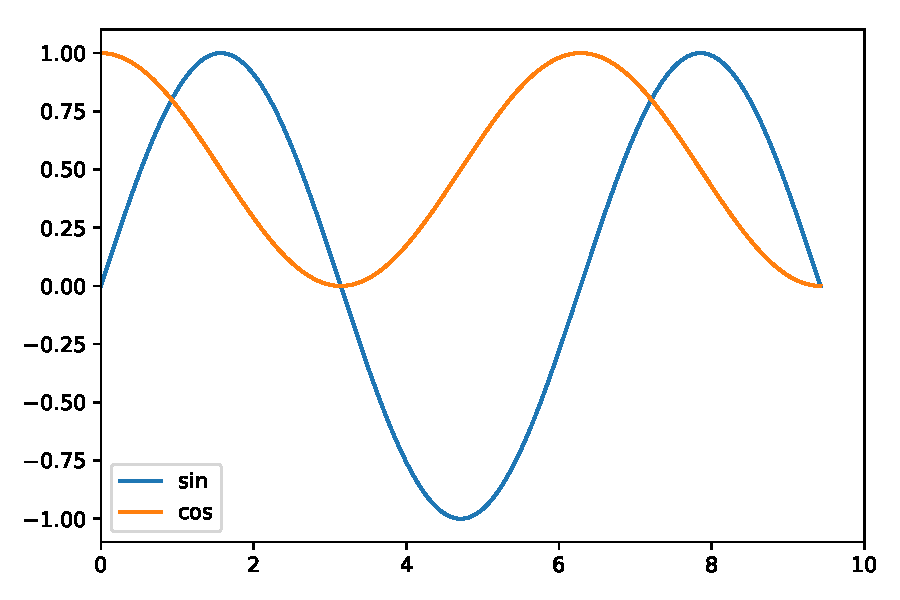
\includegraphics{demofig}
\caption{This is the caption for the figure above. Adding a label for
cross reference. \label{fig:demo}}
\end{figure}

We can refer to this figure, with \ref{fig:demo}, though the cross
reference of course doesn't work inside the notebook.



\end{document}
